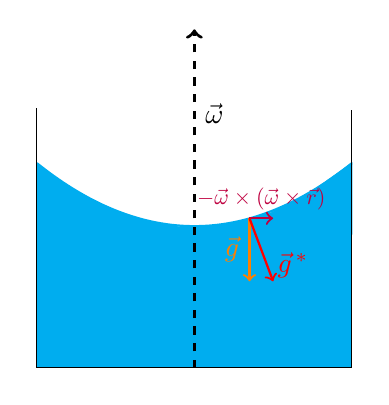
\begin{tikzpicture}

\draw [fill=cyan]  (-0.5,1.5) rectangle (3.5,-1.8) node (v4) {};
\draw [fill=white] (-0.5,1.5) rectangle (3.5,0);
\draw [white,very thick] (3.5,1.5) node (v5) {} -- (-0.5,1.5) node (v3) {};
\draw [white,very thick] (3.5,0) node (v1) {} -- (-0.5,0);
\draw[scale=1,domain=-2:2,smooth,variable=\x,cyan, thick] plot (\x+1.5, {0.2*\x*\x});
\draw [fill,cyan] (-0.5,0.8) node (v2) {} -- (-0.5,-0.1) -- (3.5,-0.1) -- (3.5,0.8) -- (2.8934,0.3692) -- (2.4713,0.1666) -- (2.0492,0.0484) -- (1.6186,-0.0107) -- (1.2978,-0.0107) -- (0.9348,0.0569) -- (0.5127,0.1835) -- (0.1918,0.327) -- (-0.2725,0.6141) -- (v2);

\draw (v3) -- (-0.5,-1.8) -- (v4) -- (v5);
\draw [->, very thick, dashed] (1.5,-1.8) -- (1.5,2.5) node [near end, right]{$\vec{\omega}$};
\draw [->, thick, orange] (2.2,0.1) node (v6) {} -- (2.2,-0.7) node[midway, left]{$\vec{g}$};
\draw [->, thick, purple] (v6.center) -- (2.5,0.1)node[midway, above, scale=0.8]{$-\vec{\omega}\times (\vec{\omega}\times \vec{r})$};
\draw [->, thick, red] (v6.center) -- (2.5,-0.7)node[near end, right]{$\vec{g}^{\,*}$};
\end{tikzpicture}